\documentclass[10pt,a4paper]{article}
\usepackage[margin=18mm,headheight=15pt]{geometry}
\usepackage[T1]{fontenc}
\usepackage{lmodern,microtype,xcolor,booktabs,tabularx,array,tikz,fancyhdr}
\usepackage[hidelinks]{hyperref}
\usetikzlibrary{arrows.meta,positioning}
\definecolor{ink}{HTML}{18394C}\definecolor{teal}{HTML}{067D85}\definecolor{pale}{HTML}{EAF5F5}\definecolor{grey}{HTML}{566571}\definecolor{amber}{HTML}{935719}
\pagestyle{fancy}\fancyhf{}\fancyhead[L]{\small\sffamily\color{grey}OPENAGENTS / HARDENING REVIEW}\fancyhead[R]{\small 27 OCT 2026}
\fancyfoot[L]{\footnotesize Synthetic tests and local observations; no production deployment.}\fancyfoot[R]{\thepage}
\setlength{\parindent}{0pt}\setlength{\parskip}{6pt}
\newcommand{\sub}[1]{\vspace{2mm}{\large\sffamily\bfseries\color{ink}#1}\par}
\newcommand{\lead}[2]{{\small\sffamily\color{teal}#1}\par{\huge\sffamily\bfseries\color{ink}#2}\par\vspace{2mm}}
\newcommand{\callout}[1]{\par\colorbox{pale}{\parbox{\dimexpr\textwidth-16pt}{\vspace{5pt}#1\vspace{5pt}}}\par}
\newcolumntype{Y}{>{\raggedright\arraybackslash}X}
\begin{document}
\lead{01 / FUNCTIONAL AND ADVERSARIAL CHECKS}{Evidence can survive a restart.\newline Delivery stays explicit.}
The existing signed exchange passes its tests. A new private observer now retains
exact receipts, deduplicates observations and tracks each recipient's delivery.
It preserves existing ownership and gates. This is the first local coordination
component, not a deployed fleet scheduler or human-signing service.

\begin{center}
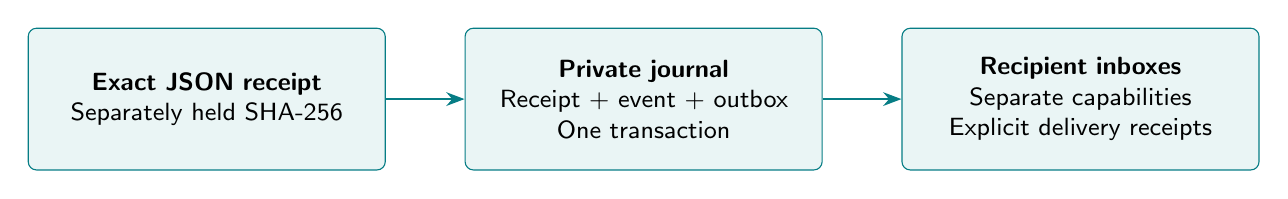
\begin{tikzpicture}[box/.style={draw=teal,fill=pale,rounded corners=3pt,text width=43mm,minimum height=18mm,align=center,font=\small\sffamily},arr/.style={-{Stealth},thick,draw=teal}]
\node[box] (r) {\textbf{Exact JSON receipt}\\Separately held SHA-256};
\node[box,right=10mm of r] (j) {\textbf{Private journal}\\Receipt + event + outbox\\One transaction};
\node[box,right=10mm of j] (i) {\textbf{Recipient inboxes}\\Separate capabilities\\Explicit delivery receipts};
\draw[arr] (r)--(j);\draw[arr] (j)--(i);
\end{tikzpicture}
\end{center}
{\footnotesize\color{grey}Implemented data flow in \texttt{integrations/workstreams}. A hash match establishes byte identity; the observer does not authenticate receipt claims or infer human awareness.}

\sub{321 tests passed locally}
\begin{tabularx}{\textwidth}{@{}Yr@{}}\toprule
\textbf{Suite} & \textbf{Passed}\\\midrule
Rust workspace, all features and locked dependencies & 167\\
Gateway / web boundary tests & 22 / 2\\
Literature / offline DFT guard and stub worker & 70 / 10\\
Actual pinned PoX adapter & 10\\
Workstream observer & 40\\\midrule
\textbf{Total} & \textbf{321}\\\bottomrule
\end{tabularx}
Gateway and web typechecks and production builds passed. Scoped federation/PoSyn
Clippy passed with warnings denied. Synthetic journeys added 27 federation,
14 PoX/Rust and 12 observer checks. No scientific calculation or live payment
was qualified by these tests. Public CI explicitly skips the five PoX tests that
require its separately installed private source.

\sub{Recovery and corruption were exercised}
Six processes submitting the same observation produce one event. Killing a
writer before commit leaves no partial event or delivery. Restart restores
pending inbox items. Capabilities cannot cross recipient or journal boundaries.
Files reject shared permissions, wrong ownership, symlinks and hardlinks; input
JSON has strict size, depth and value bounds.

Independent review found that a malformed stored timestamp could hide pending
delivery and a malformed token hash could raise a type error. Both now fail
closed before inbox filtering or authentication, with regression tests.

\callout{\textbf{A real second-machine check passed.} A second Mac ran the
40 observer tests and both observer/federation journeys. A synthetic package
signed on the first Mac was transferred with pinned hashes, verified on the
second and recorded in its observer. Signing secrets stayed on the source;
temporary canary state was removed.}

\sub{Three-host readiness remains bounded}
The intended Windows host answered SSH but rejected unattended authentication;
its worker and job state remain unverified. Current private-file handling is
Unix-only. Windows needs a qualified adapter. Two-machine tests do not establish
independent human participation, always-on operation or fleet execution authority.

\newpage
\lead{02 / DEPENDENCIES AND AUTHORITY}{Known findings addressed.\newline Remaining boundaries visible.}
\begin{tabularx}{\textwidth}{@{}Yrr@{}}\toprule
\textbf{Point-in-time advisory scan} & \textbf{Before} & \textbf{After}\\\midrule
Gateway npm production: affected package entries & 10 & 0\\
Web npm production: affected package entries & 8 & 0\\
Rust: applicable package/version findings & 5 & 0*\\
Python: 14 pinned requirements & 0 & 0\\\bottomrule
\end{tabularx}
{\footnotesize\color{grey}Evidence: \texttt{VALIDATION.json}. Counts are package entries, not unique exploits. Both full npm audits also report zero known vulnerabilities. *Rust retains one raw aggregate finding, excluded only after primary-source range review below.}

\sub{Small dependency changes, retested behavior}
The gateway stays on Express 4, now 4.22.3, with Zod 4.6.7 and patched
parser/proxy dependencies. Next is 16.4.3 with patched Sharp, PostCSS and related
dependencies. Unused optional x402 SDKs and unused web validators were removed;
live payments remain unavailable and fail closed. A new compressed-request test
confirms malformed trailing bytes produce a generic HTTP 400 and leave the
gateway responsive.

The Rust lock pins Quinn 0.11.18, Rustls 0.23.46, rustls-webpki 0.103.16,
webpki-roots 1.0.10 and Tokio 1.53.3. The updated workspace's 167 tests and scoped
Clippy passed; the federation binary was rebuilt. The final OSV scan covers
175 registry package versions. Python's 14 pinned requirements passed pip-audit
with no known vulnerabilities and no skips.

\callout{\textbf{An explicit advisory correction.} OSV's remaining raw hit treats
\texttt{block-buffer 0.10.4} as affected below 0.12.1. The maintainer explicitly
limits the affected range to \texttt{>=0.11.0,<0.12.1}. Our locked 0.10.4 is outside
that range. The raw hit and reasoning are retained; this is not a blanket package
suppression or a claim that every dependency is free of undiscovered flaws.}

\sub{CI now checks the added boundary}
Actions use verified upstream commit SHAs, checkout does not persist credentials,
token permissions remain read-only, and jobs have explicit timeouts. Linux and
macOS run observer tests and its synthetic journey; gateway and web have production
npm audit gates. Local Node 25.9 and Rust 1.89 differ from hosted Node 22 and Rust
stable, so hosted CI supplies a separate compatibility check.

\sub{Authority the observer deliberately does not acquire}
The calling OS account remains trusted. A same-account AI can access its files;
human-only acknowledgment needs a separate account or a presence-enforcing signer.
Journal hash chains detect corruption, not a malicious same-account rewrite.
Recipient tokens grant delivery access only. Records keep human awareness unknown
and receipt claims unverified; existing boards remain gate and ownership authority.

Token rotation, live backup/restore, distributed claims, execution grants, Windows
support and private push delivery remain later work. No contracts, production
services, scientific jobs or external messages were added. Private databases and
host credentials are excluded from the public branch.

\sub{Reproduce and inspect}
Run \texttt{python3 -m integrations.workstreams.demo} on Unix with Python 3.10+.
The observer README supplies CLI setup and limits. This packet includes editable
\texttt{REVIEW.md}/\texttt{REVIEW.tex}, this PDF and a source-bound validation record.
Local evidence binds exact file hashes; branch Actions provide hosted results.

{\footnotesize\color{grey}
Primary sources: \href{https://github.com/advisories/GHSA-jqcg-44mw-7w3h}{proxy-addr};
\href{https://github.com/advisories/GHSA-mrhx-c7xc-m3w5}{Zod};
\href{https://github.com/advisories/GHSA-2464-fhr4-w9xw}{Next.js};
\href{https://github.com/advisories/GHSA-27r3-jxmh-p828}{body-parser};
\href{https://github.com/RustCrypto/utils/security/advisories/GHSA-qwgh-2vcv-g2f7}{RustCrypto affected range};
\href{https://docs.github.com/en/actions/reference/security/secure-use}{GitHub secure-use guidance}.
Full details and evidence boundaries: \texttt{REVIEW.md} and \texttt{VALIDATION.json}.}
\end{document}
